\section{METHOD}
\label{chap:method}
In Subsection \ref{chap:mapping}, we discuss how the existing components of attack graph generation for a computer network are mapped to a microservice environment, and the concepts are illustrated using a small example. Then, in Subsection \ref{chap:technical}, we present the tools we use to achieve this mapping and provide an overview of the proposed system and its components, i.e., the Topology Parser (Subsection \ref{chap:topology_p}), the Vulnerability Parser (Subsection \ref{chap:vulnerability_p}), and the Attack Graph Generator (Subsection \ref{chap:attack_graph_p}). In addition, the Breath-first Search (BFS) graph traversal algorithm is discussed in Subsection \ref{chap:bfs}. 


\subsection{From Network Nodes to Microservices}
\label{chap:mapping}
% abit reptative 
In this study, we adapt existing attack graph generation methods from the computer networks field to the microservices ecosystem. To accomplish this, we identify the corresponding components and identify an equivalent replacement that can be used in a microservice architecture. In this subsection, we begin by introducing the Docker framework and its terminology. We then discuss the attack graph concepts mentioned in Subsection \ref{chap:attack_graphs} that fit our use case. We illustrate the overall concept by demonstrating a small example.

Docker is one of the most popular and used containerization frameworks currently available. In Docker, a distinction is made between the terms \textit{image}, \textit{container}, and \textit{service}. Here, an \textit{image} is an executable package that includes everything required to run an application, a \textit{container} is a runtime instance of an image, and a \textit{service} represents a container in production. A service only runs a single image, however, it codifies the way that image runs, what ports it should use, and how many replicas of the container should run so the service has the capacity it requires \cite{merkel2014docker}. We construct attack graphs by statically analyzing the topology of the containers; therefore, we treat these terms equally.  

Privileges play a central role in the generation of attack graphs. Traditionally, the privileges are modeled as a hierarchy that varies in the access level (\textit{User, Admin}), and access scope (virtual machine VOS, host machine OS). The privileges used in this paper are \textit{None, VOS(User), VOS(Admin), OS(User), and OS(Admin)}. VOS means that the privilege is exclusive to a virtual machine while not affecting the host machine. However in our case, unlike hosts in a network, these privileges refer to images and not virtual machines. The \textit{OS} keyword means that a user who has this privilege can control the host machine. Since \textit{VOSs} are isolated from host machines and their exploitation does not imply exploitation of the host machine, they are at the lower level of the hierarchy \cite{aksu2018automated}. \textit{None} means that no privilege is obtained, \textit{User} means that only a subset of user level privileges is granted, and \textit{Admin} grants control over the whole system.

As mentioned previously, \textit{nodes} and \textit{edges} are the basic building blocks of an attack graph. A \textit{node} represents a combination of a compromised Docker image and a certain privilege gained by the attacker after exploiting a vulnerability. A directed \textit{edge} between two nodes represents an attack step from one node to another (adjacent exploitable image with the gained privileges). Each edge is typed with the vulnerability (CVE) that could be exploited in the end node.

For attackers to exploit a given vulnerability, they must have certain \textit{preconditions}, i.e., the minimum privileges required to exploit \cite{aksu2018automated}. Once an attacker meets these preconditions and exploits the vulnerability, he gains the privilege of the end node as a \textit{postcondition}, and a directed edge is added between the two nodes. Both the preconditions and postconditions in this study are transformed from precondition and postcondition rules manually selected and evaluated by experts \cite{aksu2018automated}. The precondition and postcondition rules use the fields defined by the NVD, as well as an occurrence of specific keywords from CVE descriptions \cite{booth2013national}.

\subsubsection{Example}

\begin{figure*}[!h]
	\centering
	\begin{subfigure}[b]{\columnwidth}
		\centering
		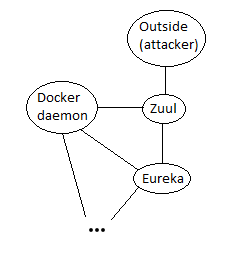
\includegraphics[width=.5\linewidth]{./images/Topology_graph}
		\caption{}
		\label{TopologyGraph}
	\end{subfigure}
	\hfill
	\begin{subfigure}[b]{\columnwidth}
		\centering
		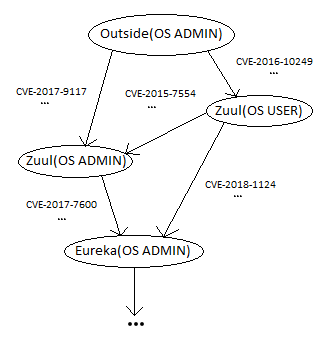
\includegraphics[width=.5\linewidth]{./images/Attack_graph}
		\caption{}
		\label{AttackGraph}
	\end{subfigure}
	
	\caption[Two numerical solutions]{Reduced Netflix OSS example: (a) example topology graph  and (b) example resulting attack graph}
\end{figure*}


Here, we present a small example to demonstrate how attack graph generation works in practice. The example is taken from the Netflix OSS GitHub repository. The Netflix OSS example is a Spring Cloud-based microservice architecture that uses the following microservices: Service Discovery (Eureka), Circuit Breaker (Hystrix), Intelligent Routing (Zuul), and Client Side Load Balancing (Ribbon). Figure \ref{TopologyGraph} shows a subset of the example topology, where each node denotes a container and each edge is a connection between two containers if one calls the other. The topology comprises an "Outside" node and a "Docker daemon" node, as well as Zuul, Eureka, and other nodes. According to Netflix, Zuul is an edge service that provides dynamic routing, monitoring, resilience, and security functionalities. Eureka is a Representational State Transfer (REST) based service primarily used in the cloud for locating services for load balancing and fail-over of middle-tier servers. Figure \ref{AttackGraph} shows a part of the corresponding attack graph, where a node is a pair of the image and its privilege, while an edge represents an atomic attack. Parts of both graphs have been omitted intentionally for simplicity. An example path an attacker would take could be to first attack the Zuul container by exploiting the CVE-2016-10249 vulnerability by crafting an image file, which triggers a heap-based buffer overflow\footnote{\url{https://nvd.nist.gov/vuln/detail/CVE-2016-10249}} and gains the USER privilege.  With this USER privilege, an attacker can exploit the CVE-2015-7554 vulnerability on the same container via crafted field data in an extension tag in a TIFF image\footnote{\url{https://nvd.nist.gov/vuln/detail/CVE-2015-7554}} to gain the ADMIN privilege. Once the ADMIN privilege has been obtained on the Zuul container, the attacker can attack the Eureka container by exploiting CVE-2017-7600 via another crafted image\footnote{\url{https://nvd.nist.gov/vuln/detail/CVE-2017-7600}} and gain the ADMIN privilege. Note that this is not the only path the attacker can take to obtain ADMIN privileges on the Eureka container. Another path would be to exploit the CVE-2018-1124 vulnerability by creating entries in the file system (procfs) by starting processes, which could result in crashes or arbitrary code execution\footnote{\url{https://nvd.nist.gov/vuln/detail/CVE-2018-1124}}. This vulnerability can be exploited by having only the USER privilege on Zuul to gain the ADMIN privileges of the Eureka container directly. Our attack graph generator shows both paths because it is of interest to identify all possible routes through which a container can be compromised.



\subsection{Attack Graph Generation for Docker Networks}
\label{chap:technical}

 Figure \ref{AttackGraphSystem} shows an overview of our attack graph generator, where the rectangles denote the main system components, the arrows indicate the flow of the system and the files are intermediate products. The proposed attack graph generator comprises three primary components, i.e., the \textit{Topology Parser}, the \textit{Vulnerability Parser}, and the \textit{Attack Graph Generator}. The Topology Parser reads the underlying topology of the system and converts it to a format required by the Attack Graph Generator. The Vulnerability Parser scans the vulnerabilities for each image, and the Attack Graph Generator generates the attack graph from the topology and vulnerabilities files. In the following, we first examine the system requirements, and then describe each component in greater detail.

The proposed generator was developed and tested for Docker 17.12.1-ce and Docker Compose 1.19.0 \cite{merkel2014docker}. Docker Compose\footnote{\url{https://docs.docker.com/compose/}} is a tool for defining the orchestration of  multi-container applications. Docker Compose provides a static configuration file that specifies the system containers, networks, and ports. Note that Clair and ClairCtl \footnote{\url{https://github.com/coreos/clair}} were used for vulnerability scanning. The generator was written in Python 3.6. Although we used specific versions of these tools, the pipe and filter structure of the generator can be easily extended to other versions of Docker-Compose, vulnerability scanners, and microservice architectures.


\begin{figure}
	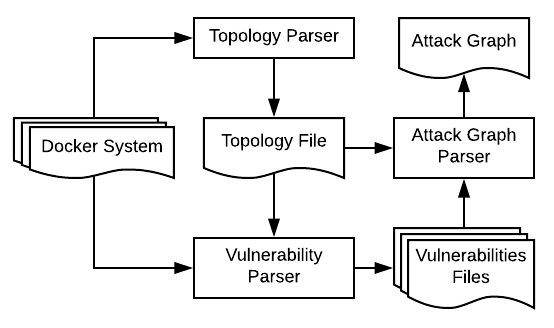
\includegraphics[scale=0.9]{./images/AttackGraphSystem}
	\caption{Overview of the proposed attach graph generator system}
	\label{AttackGraphSystem}
\end{figure}

\subsubsection{Topology Parser}
\label{chap:topology_p}

To generate an attack graph for a given system, we must arrange its components and connections as a system topology. The topology of Docker containers can be described at runtime or design time using Docker Compose. In our case, we are performing a static attack graph analysis; thus, we used Docker Compose to extract the topology. Docker Compose provides a file (docker-compose.yml) that is used to describe the orchestration of the services. In other words, this file already exists; therefore, no further input is required from a security analyst. However, different versions of the docker-compose.yml file use different syntax. For example, older versions use the deprecated keyword "\textit{link}," while newer versions exclusively use "\textit{networks}" to denote a connection between two images. Here, we use the keyword "\textit{networks}" to indicate a connection between two images.

For an application to be useful in most cases, it communicates with the outside world, i.e., it has endpoints that can be used by an outer network. In Docker, this is typically accomplished by publishing ports. This is the case for both computer networks and microservice architectures.

Another consideration is \textit{privileged access}\footnote{\url{http://obrown.io/2016/02/15/privileged-containers.html}}. In order to function properly, some containers obtain certain privileges that grant them control over the Docker daemon. For example, a user may want to run hardware (e.g., a webcam) or applications that demand higher privilege levels from Docker. In Docker, this is typically achieved either by mounting the Docker socket or specifying the "privileged" keyword in the docker-compose.yml file. Here, an attacker with access to these containers also has access to the Docker daemon. Once the attacker has access to the Docker daemon, he has potential access to the entire microservice system because each container is controlled and hosted by the daemon.

\subsubsection{Vulnerability Parser}
\label{chap:vulnerability_p}

In the preprocessing step, we use Clair to generate the vulnerabilities for a given image. Clair is a vulnerability scanner that inspects a Docker image and generates its vulnerabilities by providing a \textit{CVE-ID}, a description and an attack vector for each vulnerability. An attack vector is an entity that describes which conditions and effects are connected to the given vulnerability. We collect the fields in the attack vector as defined by the NVD \cite{booth2013national}:

\begin{itemize}
	\item Access Vector (Local, Adjacent Network, Network)
	\item Access Complexity (Low, Medium, High)
	\item Authentication (None, Single, Multiple)
	\item Confidentiality Impact (None, Partial, Complete)
	\item Integrity Impact (None, Partial, Complete)
	\item Availability Impact (None, Partial, Complete)
\end{itemize}

Since Clair does not provide a command line interface to analyze a Docker image, we use Clairctl to analyze a complete Docker image.

\begin{algorithm}
	\SetAlgoLined
	\KwData{topology, cont\_expl,
		priv\_acc}
	\KwResult{nodes, edges}
	nodes, edges, passed\_nodes = [], [], [] \\ \label{alg:init_1}
	queue = Queue() \\ \label{alg:init_2}
	queue.put("outside" + "ADMIN") \\ \label{alg:attackNodeInit}
	
	\While{! queue.isEmpty()}{ \label{alg:while}
		curr\_node = queue.get() \\ \label{alg:get_node}
		curr\_cont = get\_cont(curr\_node) \\
		curr\_priv = get\_priv(curr\_node) \\
		neighbours = topology[curr\_cont] \\
		\For{nb in neighbours}{ \label{alg:neigh}
			\If{curr\_cont == docker\_host}
			{
				end = nb + "ADMIN" \\
				create\_edge(curr\_node, end) \\ \label{alg:daemonEdge}
			}
			\If{nb == docker\_host and priv\_acc[curr\_cont]}
			{     
				end = nb + "ADMIN" \\
				create\_edge(curr\_node, end) \\ \label{alg:privEdge}
				queue.put(end) \\
				passed\_nodes.add(end)        
			}
			\If{nb != outside and nb != docker\_host}{
				precond = cont\_expl[nb][precond] \\
				postcond = cont\_expl[nb][postcond] \\
				\For{vul in vuls}{
					\If{curr\_priv > precond[vul]}{    
						end = nb + post\_cond[vul]\\
						create\_edge(curr\_node, end\_node)\\ \label{alg:addEdge}
						\If{end\_node not in passed\_nodes}{
							queue.put(end\_node)\\ \label{alg:putQueue}
							passed\_nodes.add(end\_node)
					}}
				}
			}
		}
		nodes = update\_nodes()\\
		edges = update\_edges() \\
	}
	
	\caption{BFS algorithm for attack graph generation}
	\label{BFSalgorithm}
\end{algorithm}

\subsubsection{Attack Graph Generator}
\label{chap:attack_graph_p}

After the topology is extracted and the vulnerabilities for each container are generated, we proceed to attack graph generation. Here, we first preprocess the vulnerabilities and convert them to sets of preconditions and postconditions. To achieve this, we match the previously acquired attack vectors from the vulnerability database and keywords of the descriptions of each vulnerability to generate attack rules. When a subset of attack vector fields and description keywords matches a given rule, we use the precondition or postcondition of that rule. An example precondition attack rule would be for a vulnerability to have "gain root," "gain unrestricted, root shell access" or "obtain root" in its description and the impacts from the NVD attack vector \cite{booth2013national} to be "COMPLETE" to obtain the OS(ADMIN) precondition \cite{aksu2018automated}. If more than one rule matches, we take the rule with the highest privilege level for preconditions and the lowest privilege level for postconditions. If no rule matches, we take None as the precondition and ADMIN(OS) as the postcondition. This results in a list of container vulnerabilities with their preconditions and postconditions.

\paragraph{Breadth-first Search}
\label{chap:bfs}

After preprocessing, the vulnerabilities are parsed and their preconditions and postconditions are extracted. Together with the topology, they are fed into a BFS algorithm. BFS is a popular search algorithm that traverses a graph by first looking at the neighbors of a given node before diving deeper into the graph. The pseudocode for our modified BFS algorithm is given in Algorithm \ref{BFSalgorithm}. This algorithm requires a topology, a dictionary of the exploitable vulnerabilities, and a list of nodes with privileged access as input. The output comprises nodes and edges that form the attack graph. In Algorithm \ref{BFSalgorithm}, "topology" (Subsection \ref{chap:topology_p}) provides information about the connectivity between containers, "cont\_expl" (Subsections \ref{chap:vulnerability_p} and \ref{chap:attack_graph_p}) contains information about which vulnerabilities can be attacked (with their preconditions and postconditions), and "priv\_acc" (Subsection \ref{chap:topology_p}) is an array of nodes with high (i.e., ADMIN) permissions to the Docker daemon. First, the algorithm initializes the nodes, edges, queue, and passed nodes (lines \ref{alg:init_1} and \ref{alg:init_2}). Then, it generates the attacker node (line \ref{alg:attackNodeInit}) as the node where the attack begins. The attacker node is a combination of the image name ("outside") and the privilege level (ADMIN). Then, in a while loop (line \ref{alg:while}), the algorithm iterates through each node (line \ref{alg:get_node}), checks the given node's neighbors (line \ref{alg:neigh}), and adds the edges if the conditions are satisfied (lines \ref{alg:daemonEdge}, \ref{alg:privEdge} and \ref{alg:addEdge}). If a neighbor was not passed, then it is added to the queue (line \ref{alg:putQueue}). The algorithm terminates when the queue is empty (line \ref{alg:while}). Furthermore, BFS is characterized by the following properties.


\begin{itemize}
	\item Completeness: BFS is complete, i.e., if there is a solution, BFS will find it regardless of the graph type.
	\item Termination: This follows from the monotonicity property. Monotonicity is ensured if it is assumed that an attacker will never need to relinquish a state \cite{ingols2006practical, ou2006scalable, ammann2002scalable}. In this implementation, each edge is traversed only once, which ensures that monotonicity is preserved.
	\item  Complexity: The algorithm's complexity is $O(|N| + |E|)$, where $|N|$ is the number of nodes and $|E|$ is the number of edges in the attack graph.
\end{itemize}


